\chapter{ 光电探测器单元 }
光电探测器的作用是对通信反射回来的激光束进行检测,将光能量转换为电能量,方便后续电路进行信号处理。

\section{自由光通信主要使用的探测器类型}
对于自由空间光通信系统,常用的探测器类型为光电二极管和雪崩二极管,雪崩二极管可以对十分微弱的信号进行检测,但是缺点是容易受环境噪声的影响。光电二极管是从原有的PN结基础上改良过来的,虽然没有灵敏度有所下降,但是其工作带宽高,常常应用于光纤通信系统,或使用在速率比较高的激光通信系统。

因为大气信道对激光有衰减效应,所以存在特定的大气通信波长窗口,如800nm和1550nm等,只有在该波长附近的光束才能传输更远的距离。这就要求选择对这些波长更为灵敏的光学材料,因为本课题采用的波长为1550nm,对于该波长比较灵敏的材料是铟镓砷,所以在后面选型的时候就要选择该材料作为探测单元的探测器。


\section{通信接收单元的信号处理}

\addimg{1}{digitalReceiver.pdf}{数字光接收机组成原理图}
在自由光通信系统中,由于现有激光器的功率在体积较小的情况下,基本不能做的很大,所以有激光器发射出来的光束能量本来就很小,在大气传输后,进一步削弱,导致探测器检测到信号的时候,已经非常微弱了,基本在毫伏和微伏量级,这就对探测器接收电路设计提出了更高的要求。

为了匹配现有的TTL电平标准,需要对信号进行放大,通常需要设计两级放大器进行信号的放大。探测器的材料一般基于光电导效应,探测材料经激光照射后,其导电率会发生变化,或者反映为电流的变化,所以第一级放大电路一般为电流\-电压转换型放大器,进行小信号放大,推荐使用跨阻放大器作为前端放大器;第二级放大器推荐使用线性放大器,对前置放大器进行补偿和校正,稳定输出电压。


\addimg{1}{dataregeneration.pdf}{判决与再生过程}

经过两级放大器放大后,信号幅值可以达伏级左右,但是因为在放大过程中,一并把噪声信号也进行了同等级别的放大,所以在进行时钟提取和数据恢复(如图~\ref{dataregeneration.pdf})时,需要先经过均衡滤波,即先经过滤波,去掉不需要的高频信号,提高信号检测的可靠性,如图~\ref{digitalReceiver.pdf}为一般激光通信系统光接收机的组成结构图。。



\section{实验所用的探测器简介}
% [铟镓砷光电探测器,自由空间型,带放大](https://www.thorlabs.com/newgrouppage9.cfm?objectgroup_id=4#tab-845)

%\addimg{0.5}{PDA20CS-EC-IMG.png}{PDA20CS-EC.png}
%\addimg{0.5}{PDA20CS-EC-PICTURE.jpg}{PDA20CS-EC.png}

\begin{figure}[!htbp]
	\centering
	\begin{subfigure}[c]{0.5\textwidth}
		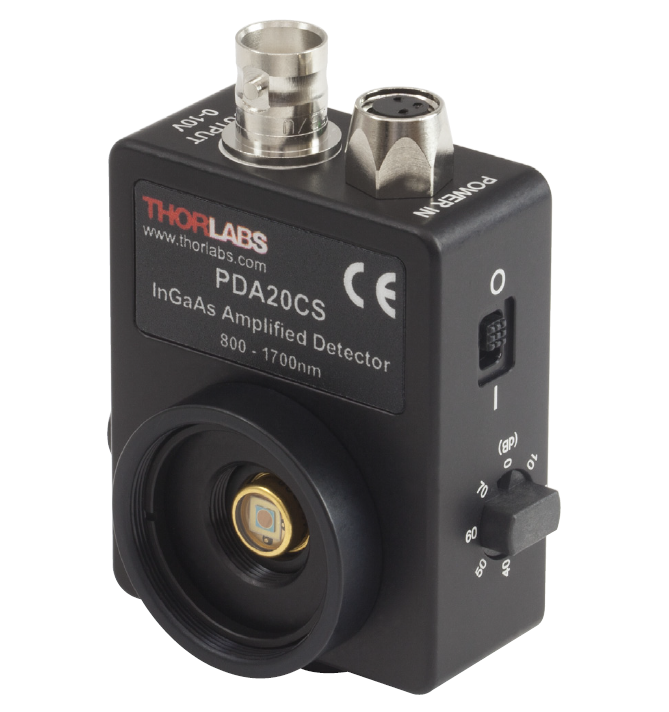
\includegraphics[width=\textwidth]{./Img/PDA20CS-EC-IMG.png}
		\caption{}
		\label{PDA20CS-EC-IMG}
	\end{subfigure}%
	~%add desired spacing
	\begin{subfigure}[c]{0.5\textwidth}
		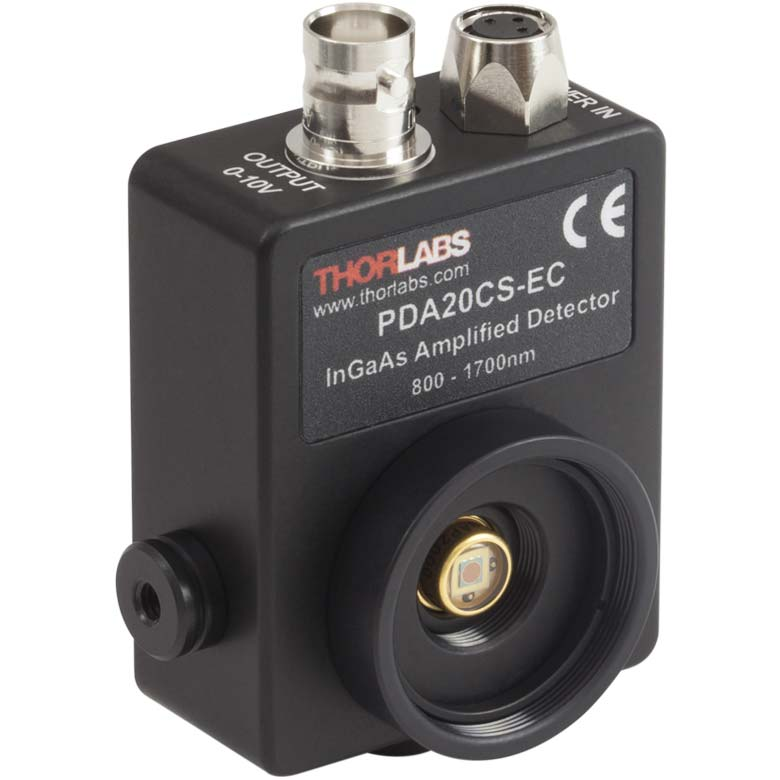
\includegraphics[width=\textwidth]{./Img/PDA20CS-EC-PICTURE.jpg}
		\caption{}
		\label{PDA20CS-EC-PICTURE}
	\end{subfigure}

	\bicaption{探测器。(a) 右侧图,(b) 左侧图}{Detector.(a) right , (b) left }
	\label{fig:PDA20CS}
\end{figure}

因为选用的激光是1550nm波长,所以探测器的材料优先选择InGaAs,该材料对该波长的激光比较灵敏,响应较快。实验采用的是THORLABS公司的铟镓砷光电探测器(自由空间型,带放大),型号为PDA20CS(-EC),带8档的增益可调节按钮。该公司提供了多种铟镓砷(InGaAs)自由空间型带放大的光电探测器,用于探测近红外波段的光。Thorlabs带放大光电探测器采用了内置低噪声跨阻放大器(TIA)的设计。


\addimg{1}{PDA20CSanzhuangtu.png}{PDA20CS安装尺寸图}
%\addimg{1}{PDA20CSTOP.jpg}{PDA20CS顶视图}
\addimg{1}{BNC-PDA20CS.png}{PDA20CS信号输出和电源管脚图}
%\addimg{1}{PDA20CFRONT.jpg}{PDA20CS正视图}

\begin{figure}[!htbp]
	\centering
	\begin{subfigure}[c]{0.5\textwidth}
		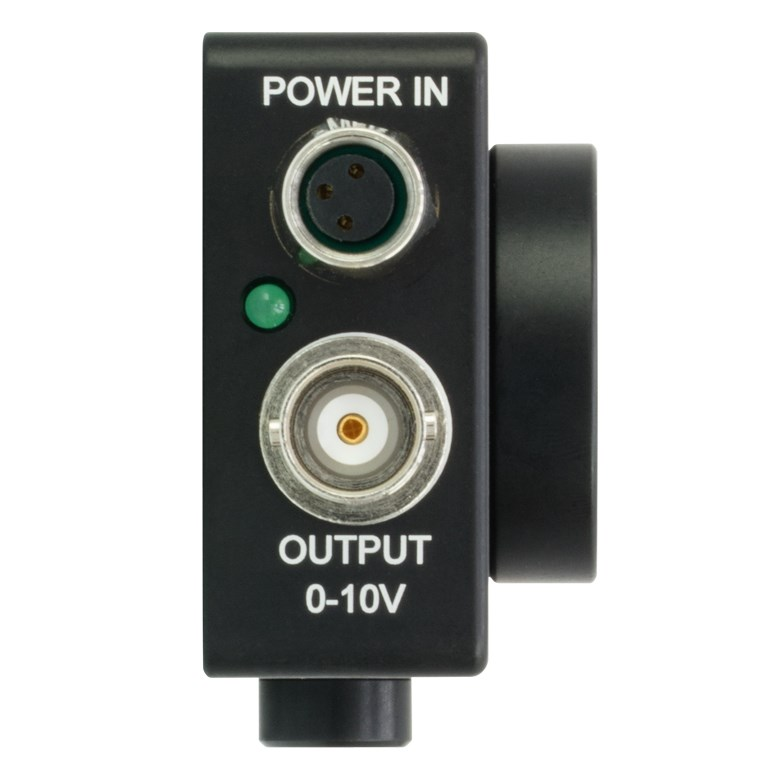
\includegraphics[width=\textwidth]{./Img/PDA20CSTOP.jpg}
		\caption{}
		\label{fig:PDA20CS-EC-IMG}
	\end{subfigure}%
	~%add desired spacing
	\begin{subfigure}[c]{0.5\textwidth}
		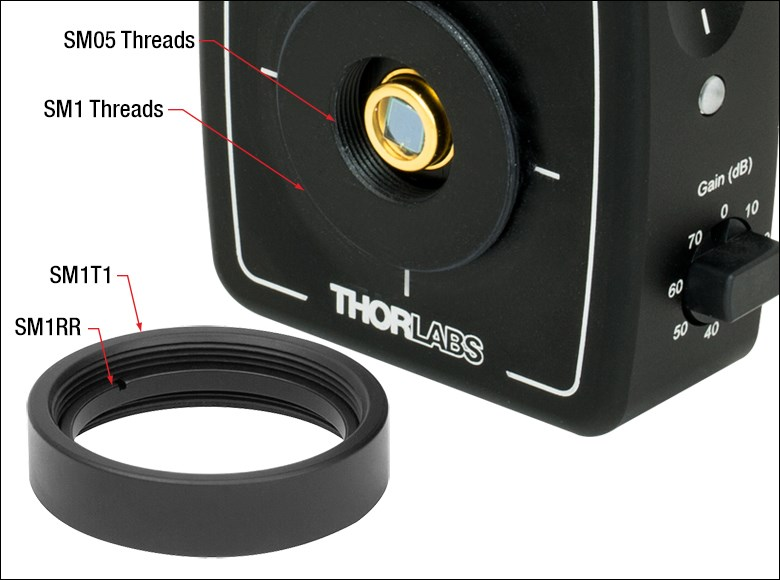
\includegraphics[width=\textwidth]{./Img/PDA20CFRONT.jpg}
		\caption{}
		\label{fig:PDA20CS-EC-PICTURE}
	\end{subfigure}
	
	\bicaption{探测器。(a) PDA20CS顶视图,(b) PDA20CS正视图}{Detector.(a) TOP VIEW , (b) FRONT VIEW }
	\label{fig:PDA20CSTOPANDFRONT}
\end{figure}

对于PDA20CS探测器的增益问题,需要注意的问题是,在平常在设计激光接收电路的时候,探测器后面需要有前置放大器,AGC放大器,最后还需要时钟提取和数据判决电路,但是PDA20CS已经集成了前置放大器和AGC放大器。

\addimg{1}{swichable-gain-and-BW.pdf}{PDA20CS增益和带宽}
\addimg{1}{swtich-gain.pdf}{PDA20CS增益参数表}
虽然图\ref{swtich-gain.pdf}表格说明了PDA20CS在高阻态使用(接示波器)的时候,可以输出0\textasciitilde10V的电压变化,而在输出口接50$ \Omega $负载电阻可以输出0\textasciitilde5V的电压变化量,但实际上这个电压输出最大值并不是每一个档位都能输出这个动态范围,比如,如果使用连续激光源和检测器增益为1(0 dB)设置时,高阻态最大输出电压为2V,而带50$ \Omega $负载时最大输出电压为1V;如果使用连续激光源和检测器增益为10 dB设置时,高阻态最大输出电压为7V,而带50$ \Omega $负载时最大输出电压为3.5V,所以在后续的时钟提取和数据提取电路需要设置相应的过压保护电路。








